% fig2-fl-ehds-architecture.tex
% FL-EHDS Three-Layer Architecture Diagram
% Grayscale version for IEEE publication
% To be placed in figures/ folder and included via % fig2-fl-ehds-architecture.tex
% FL-EHDS Three-Layer Architecture Diagram
% Grayscale version for IEEE publication
% To be placed in figures/ folder and included via % fig2-fl-ehds-architecture.tex
% FL-EHDS Three-Layer Architecture Diagram
% Grayscale version for IEEE publication
% To be placed in figures/ folder and included via % fig2-fl-ehds-architecture.tex
% FL-EHDS Three-Layer Architecture Diagram
% Grayscale version for IEEE publication
% To be placed in figures/ folder and included via \input{figures/fig2-fl-ehds-architecture}

\begin{figure*}[htbp]
\centering
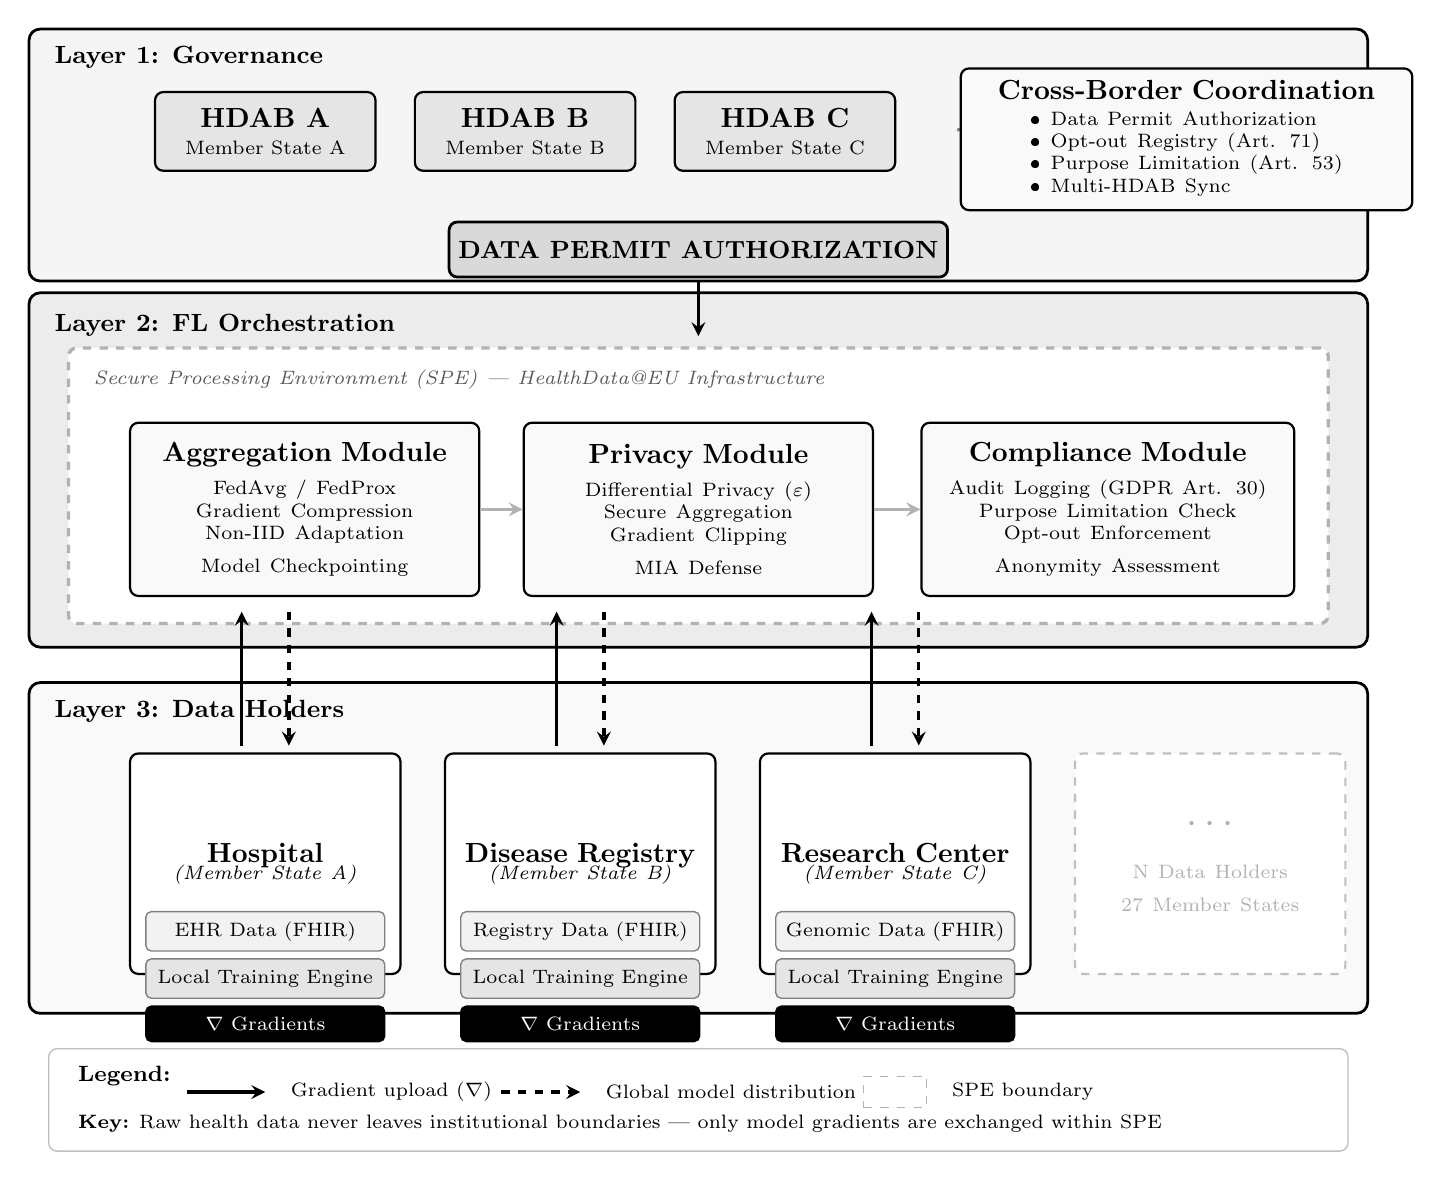
\begin{tikzpicture}[
    % Styles
    layer/.style={rectangle, rounded corners=4pt, minimum width=17cm, draw=black, line width=1pt},
    module/.style={rectangle, rounded corners=3pt, draw=black, line width=0.8pt, fill=white, minimum height=2.2cm, text width=4.2cm, align=center},
    hdab/.style={rectangle, rounded corners=3pt, draw=black, line width=0.8pt, fill=gray!20, minimum height=1cm, minimum width=2.8cm, align=center},
    dataholder/.style={rectangle, rounded corners=3pt, draw=black, line width=0.8pt, fill=white, minimum height=2.8cm, text width=3.2cm, align=center},
    databox/.style={rectangle, rounded corners=2pt, draw=gray, line width=0.5pt, fill=gray!10, minimum height=0.5cm, text width=2.8cm, align=center, font=\scriptsize},
    gradientbox/.style={rectangle, rounded corners=2pt, draw=black, line width=0.5pt, fill=black, minimum height=0.45cm, text width=2.8cm, align=center, font=\scriptsize\color{white}},
    arrow/.style={->, >=stealth, line width=1.2pt},
    dashedarrow/.style={->, >=stealth, line width=1.2pt, dashed},
    label/.style={font=\footnotesize},
    title/.style={font=\small\bfseries},
    subtitle/.style={font=\scriptsize\itshape, text=gray!70!black},
]

% ===== LAYER 1: GOVERNANCE =====
\node[layer, fill=gray!8, minimum height=3.2cm] (layer1) at (0, 8) {};
\node[title, anchor=north west] at (-8.3, 9.5) {Layer 1: Governance};

% HDABs
\node[hdab] (hdabA) at (-5.5, 8.3) {\textbf{HDAB A}\\[-2pt]\scriptsize Member State A};
\node[hdab] (hdabB) at (-2.2, 8.3) {\textbf{HDAB B}\\[-2pt]\scriptsize Member State B};
\node[hdab] (hdabC) at (1.1, 8.3) {\textbf{HDAB C}\\[-2pt]\scriptsize Member State C};
\node[font=\large, text=gray] at (3.5, 8.3) {$\cdots$};

% Coordination box
\node[module, minimum height=1.8cm, text width=5.5cm, fill=gray!5] (coord) at (6.2, 8.2) {
    \textbf{Cross-Border Coordination}\\[3pt]
    \scriptsize
    \begin{tabular}{@{}l@{}}
    • Data Permit Authorization\\
    • Opt-out Registry (Art. 71)\\
    • Purpose Limitation (Art. 53)\\
    • Multi-HDAB Sync
    \end{tabular}
};

% Data Permit box
\node[rectangle, rounded corners=3pt, draw=black, line width=1pt, fill=gray!30, minimum height=0.7cm, minimum width=5cm] (permit) at (0, 6.8) {\small\textbf{DATA PERMIT AUTHORIZATION}};

% ===== LAYER 2: FL ORCHESTRATION =====
\node[layer, fill=gray!15, minimum height=4.5cm] (layer2) at (0, 4) {};
\node[title, anchor=north west] at (-8.3, 6.1) {Layer 2: FL Orchestration};

% SPE boundary
\node[rectangle, rounded corners=3pt, draw=gray!60, line width=1.2pt, dashed, minimum width=16cm, minimum height=3.5cm, fill=white] (spe) at (0, 3.8) {};
\node[subtitle, anchor=north west] at (-7.8, 5.4) {Secure Processing Environment (SPE) — HealthData@EU Infrastructure};

% Modules
\node[module, fill=gray!5] (agg) at (-5, 3.5) {
    \textbf{Aggregation Module}\\[4pt]
    \scriptsize
    FedAvg / FedProx\\
    Gradient Compression\\
    Non-IID Adaptation\\
    Model Checkpointing
};

\node[module, fill=gray!5] (priv) at (0, 3.5) {
    \textbf{Privacy Module}\\[4pt]
    \scriptsize
    Differential Privacy ($\varepsilon$)\\
    Secure Aggregation\\
    Gradient Clipping\\
    MIA Defense
};

\node[module, fill=gray!5, text width=4.5cm] (comp) at (5.2, 3.5) {
    \textbf{Compliance Module}\\[4pt]
    \scriptsize
    Audit Logging (GDPR Art. 30)\\
    Purpose Limitation Check\\
    Opt-out Enforcement\\
    Anonymity Assessment
};

% Arrows between modules
\draw[arrow, gray!60] (agg.east) -- (priv.west);
\draw[arrow, gray!60] (priv.east) -- (comp.west);

% ===== LAYER 3: DATA HOLDERS =====
\node[layer, fill=gray!5, minimum height=4.2cm] (layer3) at (0, -0.8) {};
\node[title, anchor=north west] at (-8.3, 1.2) {Layer 3: Data Holders};

% Data holders
\node[dataholder] (hosp) at (-5.5, -1) {
    \textbf{Hospital}\\[-2pt]
    \scriptsize\textit{(Member State A)}\\[6pt]
};
\node[databox, anchor=north] at (-5.5, -1.6) {EHR Data (FHIR)};
\node[databox, anchor=north, fill=gray!20] at (-5.5, -2.2) {Local Training Engine};
\node[gradientbox, anchor=north] at (-5.5, -2.8) {$\nabla$ Gradients};

\node[dataholder] (reg) at (-1.5, -1) {
    \textbf{Disease Registry}\\[-2pt]
    \scriptsize\textit{(Member State B)}\\[6pt]
};
\node[databox, anchor=north] at (-1.5, -1.6) {Registry Data (FHIR)};
\node[databox, anchor=north, fill=gray!20] at (-1.5, -2.2) {Local Training Engine};
\node[gradientbox, anchor=north] at (-1.5, -2.8) {$\nabla$ Gradients};

\node[dataholder] (res) at (2.5, -1) {
    \textbf{Research Center}\\[-2pt]
    \scriptsize\textit{(Member State C)}\\[6pt]
};
\node[databox, anchor=north] at (2.5, -1.6) {Genomic Data (FHIR)};
\node[databox, anchor=north, fill=gray!20] at (2.5, -2.2) {Local Training Engine};
\node[gradientbox, anchor=north] at (2.5, -2.8) {$\nabla$ Gradients};

% More nodes indicator
\node[dataholder, draw=gray!50, dashed, text=gray!60] (more) at (6.5, -1) {
    \Large$\cdots$\\[8pt]
    \scriptsize N Data Holders\\
    27 Member States
};

% ===== DATA FLOW ARROWS =====
% Gradients up (solid)
\draw[arrow] (-5.8, 0.5) -- (-5.8, 2.2) node[midway, left, font=\tiny] {};
\draw[arrow] (-1.8, 0.5) -- (-1.8, 2.2);
\draw[arrow] (2.2, 0.5) -- (2.2, 2.2);

% Model down (dashed)
\draw[dashedarrow] (-5.2, 2.2) -- (-5.2, 0.5);
\draw[dashedarrow] (-1.2, 2.2) -- (-1.2, 0.5);
\draw[dashedarrow] (2.8, 2.2) -- (2.8, 0.5);

% Layer 1 to Layer 2
\draw[arrow] (0, 6.4) -- (0, 5.7);

% ===== LEGEND =====
\node[rectangle, rounded corners=3pt, draw=gray!50, line width=0.5pt, fill=white, minimum width=16.5cm, minimum height=1.3cm] at (0, -4) {};
\node[font=\footnotesize\bfseries, anchor=west] at (-8, -3.7) {Legend:};

% Gradient arrow
\draw[arrow] (-6.5, -3.9) -- (-5.5, -3.9);
\node[font=\scriptsize, anchor=west] at (-5.3, -3.9) {Gradient upload ($\nabla$)};

% Model arrow  
\draw[dashedarrow] (-2.5, -3.9) -- (-1.5, -3.9);
\node[font=\scriptsize, anchor=west] at (-1.3, -3.9) {Global model distribution};

% SPE
\node[rectangle, draw=gray!60, dashed, minimum width=0.8cm, minimum height=0.4cm] at (2.5, -3.9) {};
\node[font=\scriptsize, anchor=west] at (3.1, -3.9) {SPE boundary};

% Key principle
\node[font=\scriptsize, anchor=west] at (-8, -4.3) {\textbf{Key:} Raw health data never leaves institutional boundaries — only model gradients are exchanged within SPE};

\end{tikzpicture}
\caption{FL-EHDS three-layer compliance framework architecture. Layer~1 (Governance) integrates Health Data Access Bodies for cross-border data permit authorization and opt-out registry consultation per Article~71. Layer~2 (FL Orchestration) operates within a Secure Processing Environment, implementing gradient aggregation with FedAvg/FedProx, privacy protection via differential privacy and secure aggregation, and GDPR-compliant audit logging. Layer~3 (Data Holders) maintains raw data within institutional boundaries across 27 Member States; only gradients ($\nabla$) are transmitted upward while global model parameters flow downward.}
\label{fig:architecture}
\end{figure*}


\begin{figure*}[htbp]
\centering
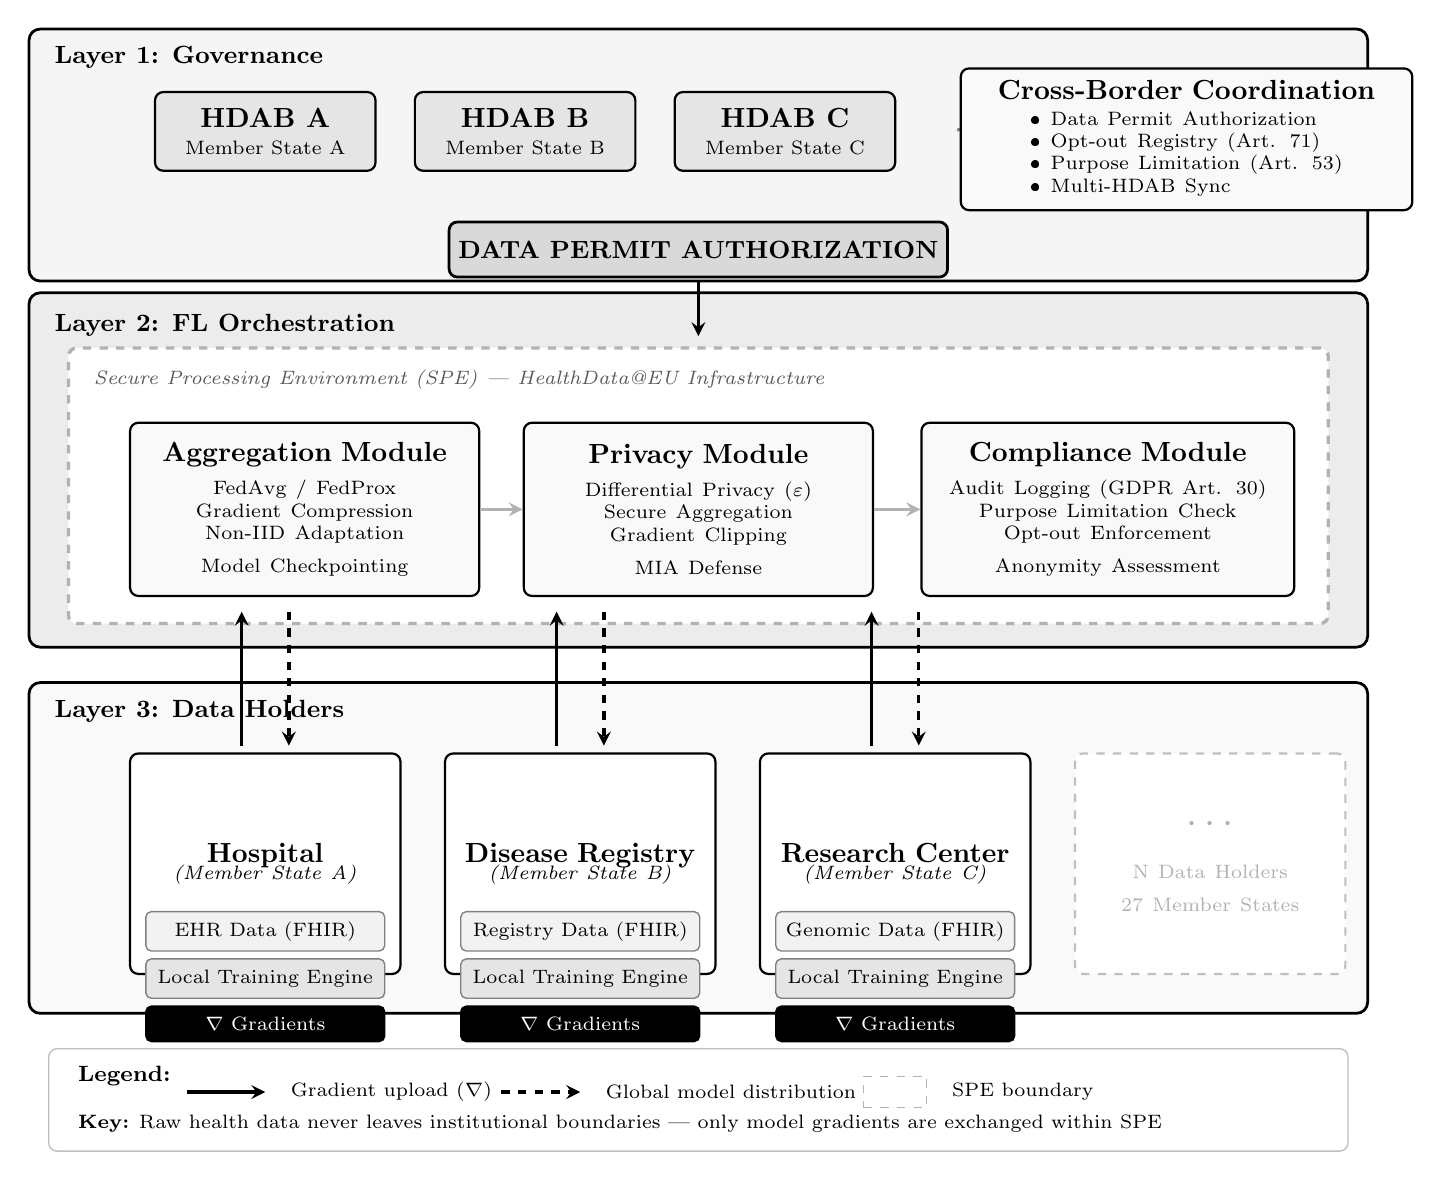
\begin{tikzpicture}[
    % Styles
    layer/.style={rectangle, rounded corners=4pt, minimum width=17cm, draw=black, line width=1pt},
    module/.style={rectangle, rounded corners=3pt, draw=black, line width=0.8pt, fill=white, minimum height=2.2cm, text width=4.2cm, align=center},
    hdab/.style={rectangle, rounded corners=3pt, draw=black, line width=0.8pt, fill=gray!20, minimum height=1cm, minimum width=2.8cm, align=center},
    dataholder/.style={rectangle, rounded corners=3pt, draw=black, line width=0.8pt, fill=white, minimum height=2.8cm, text width=3.2cm, align=center},
    databox/.style={rectangle, rounded corners=2pt, draw=gray, line width=0.5pt, fill=gray!10, minimum height=0.5cm, text width=2.8cm, align=center, font=\scriptsize},
    gradientbox/.style={rectangle, rounded corners=2pt, draw=black, line width=0.5pt, fill=black, minimum height=0.45cm, text width=2.8cm, align=center, font=\scriptsize\color{white}},
    arrow/.style={->, >=stealth, line width=1.2pt},
    dashedarrow/.style={->, >=stealth, line width=1.2pt, dashed},
    label/.style={font=\footnotesize},
    title/.style={font=\small\bfseries},
    subtitle/.style={font=\scriptsize\itshape, text=gray!70!black},
]

% ===== LAYER 1: GOVERNANCE =====
\node[layer, fill=gray!8, minimum height=3.2cm] (layer1) at (0, 8) {};
\node[title, anchor=north west] at (-8.3, 9.5) {Layer 1: Governance};

% HDABs
\node[hdab] (hdabA) at (-5.5, 8.3) {\textbf{HDAB A}\\[-2pt]\scriptsize Member State A};
\node[hdab] (hdabB) at (-2.2, 8.3) {\textbf{HDAB B}\\[-2pt]\scriptsize Member State B};
\node[hdab] (hdabC) at (1.1, 8.3) {\textbf{HDAB C}\\[-2pt]\scriptsize Member State C};
\node[font=\large, text=gray] at (3.5, 8.3) {$\cdots$};

% Coordination box
\node[module, minimum height=1.8cm, text width=5.5cm, fill=gray!5] (coord) at (6.2, 8.2) {
    \textbf{Cross-Border Coordination}\\[3pt]
    \scriptsize
    \begin{tabular}{@{}l@{}}
    • Data Permit Authorization\\
    • Opt-out Registry (Art. 71)\\
    • Purpose Limitation (Art. 53)\\
    • Multi-HDAB Sync
    \end{tabular}
};

% Data Permit box
\node[rectangle, rounded corners=3pt, draw=black, line width=1pt, fill=gray!30, minimum height=0.7cm, minimum width=5cm] (permit) at (0, 6.8) {\small\textbf{DATA PERMIT AUTHORIZATION}};

% ===== LAYER 2: FL ORCHESTRATION =====
\node[layer, fill=gray!15, minimum height=4.5cm] (layer2) at (0, 4) {};
\node[title, anchor=north west] at (-8.3, 6.1) {Layer 2: FL Orchestration};

% SPE boundary
\node[rectangle, rounded corners=3pt, draw=gray!60, line width=1.2pt, dashed, minimum width=16cm, minimum height=3.5cm, fill=white] (spe) at (0, 3.8) {};
\node[subtitle, anchor=north west] at (-7.8, 5.4) {Secure Processing Environment (SPE) — HealthData@EU Infrastructure};

% Modules
\node[module, fill=gray!5] (agg) at (-5, 3.5) {
    \textbf{Aggregation Module}\\[4pt]
    \scriptsize
    FedAvg / FedProx\\
    Gradient Compression\\
    Non-IID Adaptation\\
    Model Checkpointing
};

\node[module, fill=gray!5] (priv) at (0, 3.5) {
    \textbf{Privacy Module}\\[4pt]
    \scriptsize
    Differential Privacy ($\varepsilon$)\\
    Secure Aggregation\\
    Gradient Clipping\\
    MIA Defense
};

\node[module, fill=gray!5, text width=4.5cm] (comp) at (5.2, 3.5) {
    \textbf{Compliance Module}\\[4pt]
    \scriptsize
    Audit Logging (GDPR Art. 30)\\
    Purpose Limitation Check\\
    Opt-out Enforcement\\
    Anonymity Assessment
};

% Arrows between modules
\draw[arrow, gray!60] (agg.east) -- (priv.west);
\draw[arrow, gray!60] (priv.east) -- (comp.west);

% ===== LAYER 3: DATA HOLDERS =====
\node[layer, fill=gray!5, minimum height=4.2cm] (layer3) at (0, -0.8) {};
\node[title, anchor=north west] at (-8.3, 1.2) {Layer 3: Data Holders};

% Data holders
\node[dataholder] (hosp) at (-5.5, -1) {
    \textbf{Hospital}\\[-2pt]
    \scriptsize\textit{(Member State A)}\\[6pt]
};
\node[databox, anchor=north] at (-5.5, -1.6) {EHR Data (FHIR)};
\node[databox, anchor=north, fill=gray!20] at (-5.5, -2.2) {Local Training Engine};
\node[gradientbox, anchor=north] at (-5.5, -2.8) {$\nabla$ Gradients};

\node[dataholder] (reg) at (-1.5, -1) {
    \textbf{Disease Registry}\\[-2pt]
    \scriptsize\textit{(Member State B)}\\[6pt]
};
\node[databox, anchor=north] at (-1.5, -1.6) {Registry Data (FHIR)};
\node[databox, anchor=north, fill=gray!20] at (-1.5, -2.2) {Local Training Engine};
\node[gradientbox, anchor=north] at (-1.5, -2.8) {$\nabla$ Gradients};

\node[dataholder] (res) at (2.5, -1) {
    \textbf{Research Center}\\[-2pt]
    \scriptsize\textit{(Member State C)}\\[6pt]
};
\node[databox, anchor=north] at (2.5, -1.6) {Genomic Data (FHIR)};
\node[databox, anchor=north, fill=gray!20] at (2.5, -2.2) {Local Training Engine};
\node[gradientbox, anchor=north] at (2.5, -2.8) {$\nabla$ Gradients};

% More nodes indicator
\node[dataholder, draw=gray!50, dashed, text=gray!60] (more) at (6.5, -1) {
    \Large$\cdots$\\[8pt]
    \scriptsize N Data Holders\\
    27 Member States
};

% ===== DATA FLOW ARROWS =====
% Gradients up (solid)
\draw[arrow] (-5.8, 0.5) -- (-5.8, 2.2) node[midway, left, font=\tiny] {};
\draw[arrow] (-1.8, 0.5) -- (-1.8, 2.2);
\draw[arrow] (2.2, 0.5) -- (2.2, 2.2);

% Model down (dashed)
\draw[dashedarrow] (-5.2, 2.2) -- (-5.2, 0.5);
\draw[dashedarrow] (-1.2, 2.2) -- (-1.2, 0.5);
\draw[dashedarrow] (2.8, 2.2) -- (2.8, 0.5);

% Layer 1 to Layer 2
\draw[arrow] (0, 6.4) -- (0, 5.7);

% ===== LEGEND =====
\node[rectangle, rounded corners=3pt, draw=gray!50, line width=0.5pt, fill=white, minimum width=16.5cm, minimum height=1.3cm] at (0, -4) {};
\node[font=\footnotesize\bfseries, anchor=west] at (-8, -3.7) {Legend:};

% Gradient arrow
\draw[arrow] (-6.5, -3.9) -- (-5.5, -3.9);
\node[font=\scriptsize, anchor=west] at (-5.3, -3.9) {Gradient upload ($\nabla$)};

% Model arrow  
\draw[dashedarrow] (-2.5, -3.9) -- (-1.5, -3.9);
\node[font=\scriptsize, anchor=west] at (-1.3, -3.9) {Global model distribution};

% SPE
\node[rectangle, draw=gray!60, dashed, minimum width=0.8cm, minimum height=0.4cm] at (2.5, -3.9) {};
\node[font=\scriptsize, anchor=west] at (3.1, -3.9) {SPE boundary};

% Key principle
\node[font=\scriptsize, anchor=west] at (-8, -4.3) {\textbf{Key:} Raw health data never leaves institutional boundaries — only model gradients are exchanged within SPE};

\end{tikzpicture}
\caption{FL-EHDS three-layer compliance framework architecture. Layer~1 (Governance) integrates Health Data Access Bodies for cross-border data permit authorization and opt-out registry consultation per Article~71. Layer~2 (FL Orchestration) operates within a Secure Processing Environment, implementing gradient aggregation with FedAvg/FedProx, privacy protection via differential privacy and secure aggregation, and GDPR-compliant audit logging. Layer~3 (Data Holders) maintains raw data within institutional boundaries across 27 Member States; only gradients ($\nabla$) are transmitted upward while global model parameters flow downward.}
\label{fig:architecture}
\end{figure*}


\begin{figure*}[htbp]
\centering
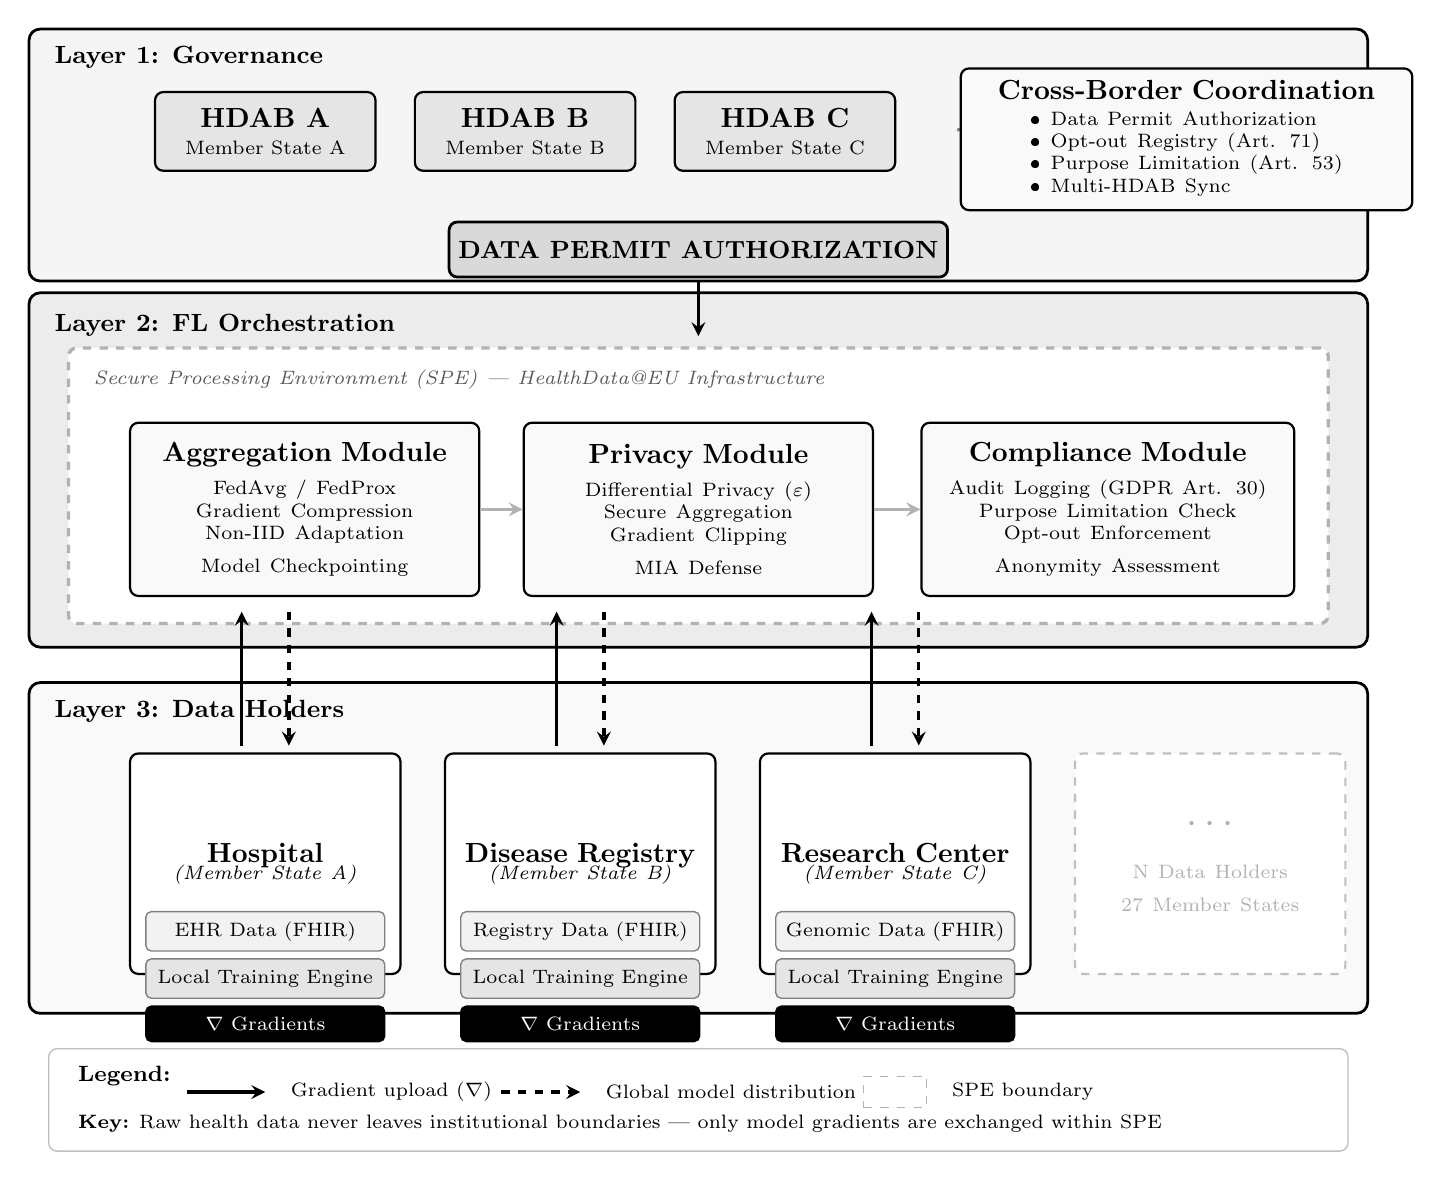
\begin{tikzpicture}[
    % Styles
    layer/.style={rectangle, rounded corners=4pt, minimum width=17cm, draw=black, line width=1pt},
    module/.style={rectangle, rounded corners=3pt, draw=black, line width=0.8pt, fill=white, minimum height=2.2cm, text width=4.2cm, align=center},
    hdab/.style={rectangle, rounded corners=3pt, draw=black, line width=0.8pt, fill=gray!20, minimum height=1cm, minimum width=2.8cm, align=center},
    dataholder/.style={rectangle, rounded corners=3pt, draw=black, line width=0.8pt, fill=white, minimum height=2.8cm, text width=3.2cm, align=center},
    databox/.style={rectangle, rounded corners=2pt, draw=gray, line width=0.5pt, fill=gray!10, minimum height=0.5cm, text width=2.8cm, align=center, font=\scriptsize},
    gradientbox/.style={rectangle, rounded corners=2pt, draw=black, line width=0.5pt, fill=black, minimum height=0.45cm, text width=2.8cm, align=center, font=\scriptsize\color{white}},
    arrow/.style={->, >=stealth, line width=1.2pt},
    dashedarrow/.style={->, >=stealth, line width=1.2pt, dashed},
    label/.style={font=\footnotesize},
    title/.style={font=\small\bfseries},
    subtitle/.style={font=\scriptsize\itshape, text=gray!70!black},
]

% ===== LAYER 1: GOVERNANCE =====
\node[layer, fill=gray!8, minimum height=3.2cm] (layer1) at (0, 8) {};
\node[title, anchor=north west] at (-8.3, 9.5) {Layer 1: Governance};

% HDABs
\node[hdab] (hdabA) at (-5.5, 8.3) {\textbf{HDAB A}\\[-2pt]\scriptsize Member State A};
\node[hdab] (hdabB) at (-2.2, 8.3) {\textbf{HDAB B}\\[-2pt]\scriptsize Member State B};
\node[hdab] (hdabC) at (1.1, 8.3) {\textbf{HDAB C}\\[-2pt]\scriptsize Member State C};
\node[font=\large, text=gray] at (3.5, 8.3) {$\cdots$};

% Coordination box
\node[module, minimum height=1.8cm, text width=5.5cm, fill=gray!5] (coord) at (6.2, 8.2) {
    \textbf{Cross-Border Coordination}\\[3pt]
    \scriptsize
    \begin{tabular}{@{}l@{}}
    • Data Permit Authorization\\
    • Opt-out Registry (Art. 71)\\
    • Purpose Limitation (Art. 53)\\
    • Multi-HDAB Sync
    \end{tabular}
};

% Data Permit box
\node[rectangle, rounded corners=3pt, draw=black, line width=1pt, fill=gray!30, minimum height=0.7cm, minimum width=5cm] (permit) at (0, 6.8) {\small\textbf{DATA PERMIT AUTHORIZATION}};

% ===== LAYER 2: FL ORCHESTRATION =====
\node[layer, fill=gray!15, minimum height=4.5cm] (layer2) at (0, 4) {};
\node[title, anchor=north west] at (-8.3, 6.1) {Layer 2: FL Orchestration};

% SPE boundary
\node[rectangle, rounded corners=3pt, draw=gray!60, line width=1.2pt, dashed, minimum width=16cm, minimum height=3.5cm, fill=white] (spe) at (0, 3.8) {};
\node[subtitle, anchor=north west] at (-7.8, 5.4) {Secure Processing Environment (SPE) — HealthData@EU Infrastructure};

% Modules
\node[module, fill=gray!5] (agg) at (-5, 3.5) {
    \textbf{Aggregation Module}\\[4pt]
    \scriptsize
    FedAvg / FedProx\\
    Gradient Compression\\
    Non-IID Adaptation\\
    Model Checkpointing
};

\node[module, fill=gray!5] (priv) at (0, 3.5) {
    \textbf{Privacy Module}\\[4pt]
    \scriptsize
    Differential Privacy ($\varepsilon$)\\
    Secure Aggregation\\
    Gradient Clipping\\
    MIA Defense
};

\node[module, fill=gray!5, text width=4.5cm] (comp) at (5.2, 3.5) {
    \textbf{Compliance Module}\\[4pt]
    \scriptsize
    Audit Logging (GDPR Art. 30)\\
    Purpose Limitation Check\\
    Opt-out Enforcement\\
    Anonymity Assessment
};

% Arrows between modules
\draw[arrow, gray!60] (agg.east) -- (priv.west);
\draw[arrow, gray!60] (priv.east) -- (comp.west);

% ===== LAYER 3: DATA HOLDERS =====
\node[layer, fill=gray!5, minimum height=4.2cm] (layer3) at (0, -0.8) {};
\node[title, anchor=north west] at (-8.3, 1.2) {Layer 3: Data Holders};

% Data holders
\node[dataholder] (hosp) at (-5.5, -1) {
    \textbf{Hospital}\\[-2pt]
    \scriptsize\textit{(Member State A)}\\[6pt]
};
\node[databox, anchor=north] at (-5.5, -1.6) {EHR Data (FHIR)};
\node[databox, anchor=north, fill=gray!20] at (-5.5, -2.2) {Local Training Engine};
\node[gradientbox, anchor=north] at (-5.5, -2.8) {$\nabla$ Gradients};

\node[dataholder] (reg) at (-1.5, -1) {
    \textbf{Disease Registry}\\[-2pt]
    \scriptsize\textit{(Member State B)}\\[6pt]
};
\node[databox, anchor=north] at (-1.5, -1.6) {Registry Data (FHIR)};
\node[databox, anchor=north, fill=gray!20] at (-1.5, -2.2) {Local Training Engine};
\node[gradientbox, anchor=north] at (-1.5, -2.8) {$\nabla$ Gradients};

\node[dataholder] (res) at (2.5, -1) {
    \textbf{Research Center}\\[-2pt]
    \scriptsize\textit{(Member State C)}\\[6pt]
};
\node[databox, anchor=north] at (2.5, -1.6) {Genomic Data (FHIR)};
\node[databox, anchor=north, fill=gray!20] at (2.5, -2.2) {Local Training Engine};
\node[gradientbox, anchor=north] at (2.5, -2.8) {$\nabla$ Gradients};

% More nodes indicator
\node[dataholder, draw=gray!50, dashed, text=gray!60] (more) at (6.5, -1) {
    \Large$\cdots$\\[8pt]
    \scriptsize N Data Holders\\
    27 Member States
};

% ===== DATA FLOW ARROWS =====
% Gradients up (solid)
\draw[arrow] (-5.8, 0.5) -- (-5.8, 2.2) node[midway, left, font=\tiny] {};
\draw[arrow] (-1.8, 0.5) -- (-1.8, 2.2);
\draw[arrow] (2.2, 0.5) -- (2.2, 2.2);

% Model down (dashed)
\draw[dashedarrow] (-5.2, 2.2) -- (-5.2, 0.5);
\draw[dashedarrow] (-1.2, 2.2) -- (-1.2, 0.5);
\draw[dashedarrow] (2.8, 2.2) -- (2.8, 0.5);

% Layer 1 to Layer 2
\draw[arrow] (0, 6.4) -- (0, 5.7);

% ===== LEGEND =====
\node[rectangle, rounded corners=3pt, draw=gray!50, line width=0.5pt, fill=white, minimum width=16.5cm, minimum height=1.3cm] at (0, -4) {};
\node[font=\footnotesize\bfseries, anchor=west] at (-8, -3.7) {Legend:};

% Gradient arrow
\draw[arrow] (-6.5, -3.9) -- (-5.5, -3.9);
\node[font=\scriptsize, anchor=west] at (-5.3, -3.9) {Gradient upload ($\nabla$)};

% Model arrow  
\draw[dashedarrow] (-2.5, -3.9) -- (-1.5, -3.9);
\node[font=\scriptsize, anchor=west] at (-1.3, -3.9) {Global model distribution};

% SPE
\node[rectangle, draw=gray!60, dashed, minimum width=0.8cm, minimum height=0.4cm] at (2.5, -3.9) {};
\node[font=\scriptsize, anchor=west] at (3.1, -3.9) {SPE boundary};

% Key principle
\node[font=\scriptsize, anchor=west] at (-8, -4.3) {\textbf{Key:} Raw health data never leaves institutional boundaries — only model gradients are exchanged within SPE};

\end{tikzpicture}
\caption{FL-EHDS three-layer compliance framework architecture. Layer~1 (Governance) integrates Health Data Access Bodies for cross-border data permit authorization and opt-out registry consultation per Article~71. Layer~2 (FL Orchestration) operates within a Secure Processing Environment, implementing gradient aggregation with FedAvg/FedProx, privacy protection via differential privacy and secure aggregation, and GDPR-compliant audit logging. Layer~3 (Data Holders) maintains raw data within institutional boundaries across 27 Member States; only gradients ($\nabla$) are transmitted upward while global model parameters flow downward.}
\label{fig:architecture}
\end{figure*}


\begin{figure*}[htbp]
\centering
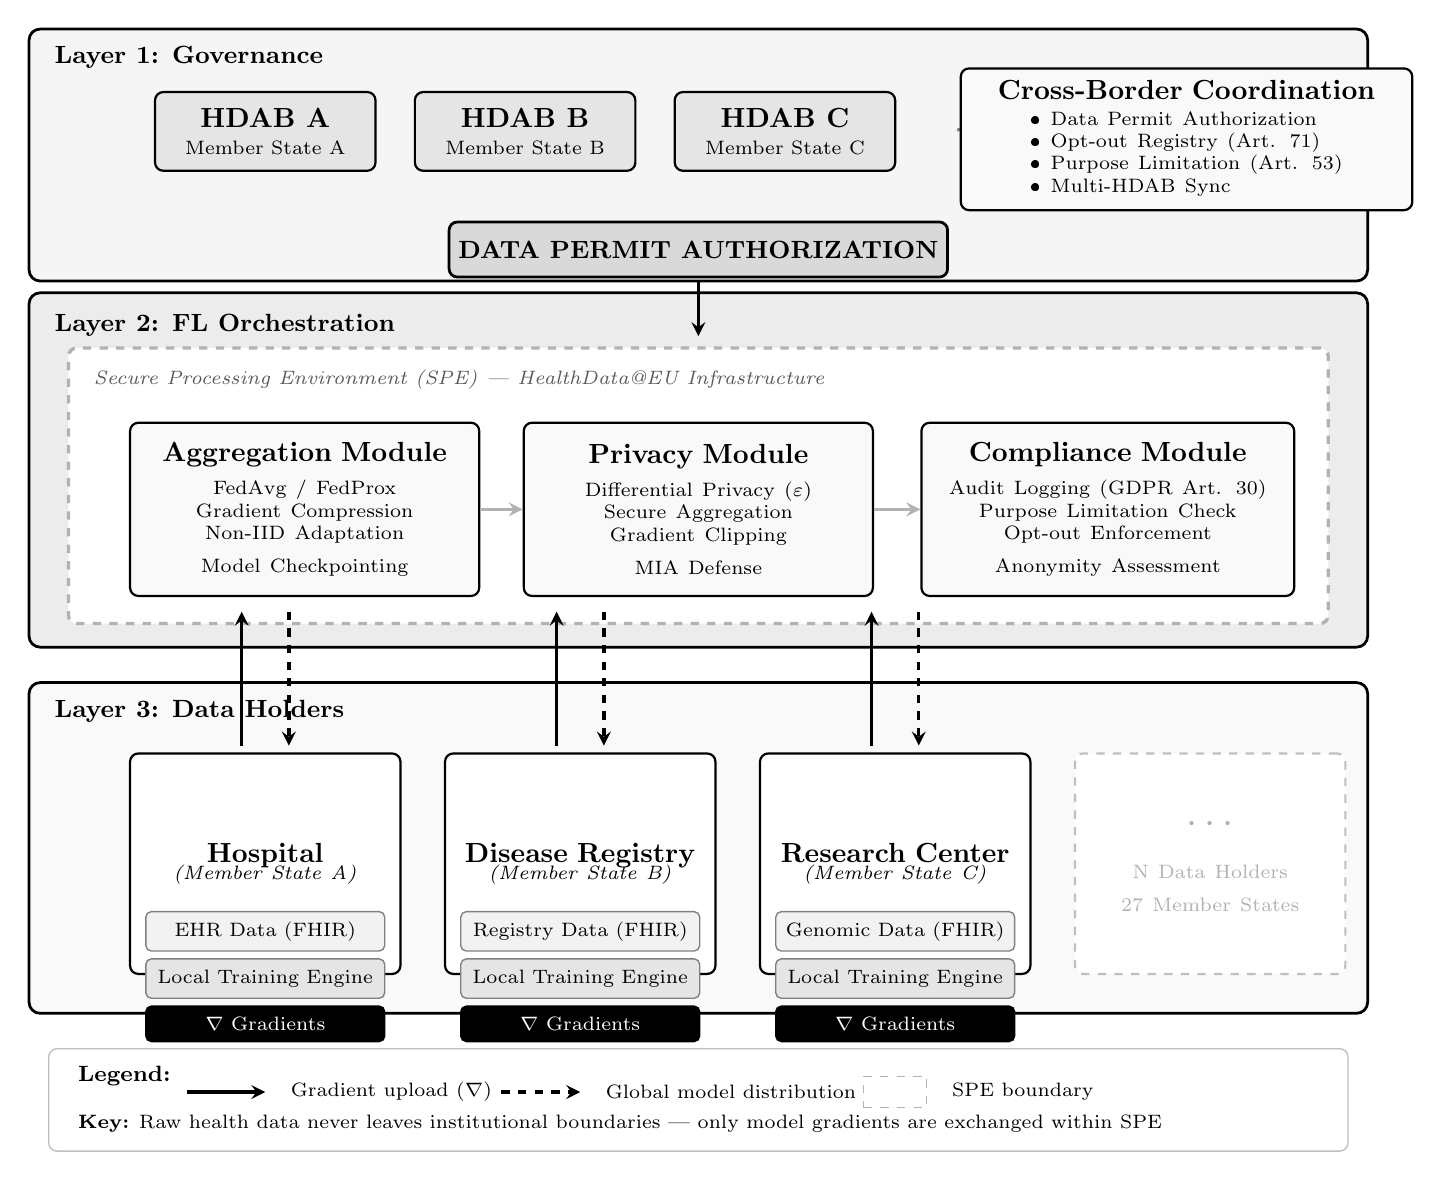
\begin{tikzpicture}[
    % Styles
    layer/.style={rectangle, rounded corners=4pt, minimum width=17cm, draw=black, line width=1pt},
    module/.style={rectangle, rounded corners=3pt, draw=black, line width=0.8pt, fill=white, minimum height=2.2cm, text width=4.2cm, align=center},
    hdab/.style={rectangle, rounded corners=3pt, draw=black, line width=0.8pt, fill=gray!20, minimum height=1cm, minimum width=2.8cm, align=center},
    dataholder/.style={rectangle, rounded corners=3pt, draw=black, line width=0.8pt, fill=white, minimum height=2.8cm, text width=3.2cm, align=center},
    databox/.style={rectangle, rounded corners=2pt, draw=gray, line width=0.5pt, fill=gray!10, minimum height=0.5cm, text width=2.8cm, align=center, font=\scriptsize},
    gradientbox/.style={rectangle, rounded corners=2pt, draw=black, line width=0.5pt, fill=black, minimum height=0.45cm, text width=2.8cm, align=center, font=\scriptsize\color{white}},
    arrow/.style={->, >=stealth, line width=1.2pt},
    dashedarrow/.style={->, >=stealth, line width=1.2pt, dashed},
    label/.style={font=\footnotesize},
    title/.style={font=\small\bfseries},
    subtitle/.style={font=\scriptsize\itshape, text=gray!70!black},
]

% ===== LAYER 1: GOVERNANCE =====
\node[layer, fill=gray!8, minimum height=3.2cm] (layer1) at (0, 8) {};
\node[title, anchor=north west] at (-8.3, 9.5) {Layer 1: Governance};

% HDABs
\node[hdab] (hdabA) at (-5.5, 8.3) {\textbf{HDAB A}\\[-2pt]\scriptsize Member State A};
\node[hdab] (hdabB) at (-2.2, 8.3) {\textbf{HDAB B}\\[-2pt]\scriptsize Member State B};
\node[hdab] (hdabC) at (1.1, 8.3) {\textbf{HDAB C}\\[-2pt]\scriptsize Member State C};
\node[font=\large, text=gray] at (3.5, 8.3) {$\cdots$};

% Coordination box
\node[module, minimum height=1.8cm, text width=5.5cm, fill=gray!5] (coord) at (6.2, 8.2) {
    \textbf{Cross-Border Coordination}\\[3pt]
    \scriptsize
    \begin{tabular}{@{}l@{}}
    • Data Permit Authorization\\
    • Opt-out Registry (Art. 71)\\
    • Purpose Limitation (Art. 53)\\
    • Multi-HDAB Sync
    \end{tabular}
};

% Data Permit box
\node[rectangle, rounded corners=3pt, draw=black, line width=1pt, fill=gray!30, minimum height=0.7cm, minimum width=5cm] (permit) at (0, 6.8) {\small\textbf{DATA PERMIT AUTHORIZATION}};

% ===== LAYER 2: FL ORCHESTRATION =====
\node[layer, fill=gray!15, minimum height=4.5cm] (layer2) at (0, 4) {};
\node[title, anchor=north west] at (-8.3, 6.1) {Layer 2: FL Orchestration};

% SPE boundary
\node[rectangle, rounded corners=3pt, draw=gray!60, line width=1.2pt, dashed, minimum width=16cm, minimum height=3.5cm, fill=white] (spe) at (0, 3.8) {};
\node[subtitle, anchor=north west] at (-7.8, 5.4) {Secure Processing Environment (SPE) — HealthData@EU Infrastructure};

% Modules
\node[module, fill=gray!5] (agg) at (-5, 3.5) {
    \textbf{Aggregation Module}\\[4pt]
    \scriptsize
    FedAvg / FedProx\\
    Gradient Compression\\
    Non-IID Adaptation\\
    Model Checkpointing
};

\node[module, fill=gray!5] (priv) at (0, 3.5) {
    \textbf{Privacy Module}\\[4pt]
    \scriptsize
    Differential Privacy ($\varepsilon$)\\
    Secure Aggregation\\
    Gradient Clipping\\
    MIA Defense
};

\node[module, fill=gray!5, text width=4.5cm] (comp) at (5.2, 3.5) {
    \textbf{Compliance Module}\\[4pt]
    \scriptsize
    Audit Logging (GDPR Art. 30)\\
    Purpose Limitation Check\\
    Opt-out Enforcement\\
    Anonymity Assessment
};

% Arrows between modules
\draw[arrow, gray!60] (agg.east) -- (priv.west);
\draw[arrow, gray!60] (priv.east) -- (comp.west);

% ===== LAYER 3: DATA HOLDERS =====
\node[layer, fill=gray!5, minimum height=4.2cm] (layer3) at (0, -0.8) {};
\node[title, anchor=north west] at (-8.3, 1.2) {Layer 3: Data Holders};

% Data holders
\node[dataholder] (hosp) at (-5.5, -1) {
    \textbf{Hospital}\\[-2pt]
    \scriptsize\textit{(Member State A)}\\[6pt]
};
\node[databox, anchor=north] at (-5.5, -1.6) {EHR Data (FHIR)};
\node[databox, anchor=north, fill=gray!20] at (-5.5, -2.2) {Local Training Engine};
\node[gradientbox, anchor=north] at (-5.5, -2.8) {$\nabla$ Gradients};

\node[dataholder] (reg) at (-1.5, -1) {
    \textbf{Disease Registry}\\[-2pt]
    \scriptsize\textit{(Member State B)}\\[6pt]
};
\node[databox, anchor=north] at (-1.5, -1.6) {Registry Data (FHIR)};
\node[databox, anchor=north, fill=gray!20] at (-1.5, -2.2) {Local Training Engine};
\node[gradientbox, anchor=north] at (-1.5, -2.8) {$\nabla$ Gradients};

\node[dataholder] (res) at (2.5, -1) {
    \textbf{Research Center}\\[-2pt]
    \scriptsize\textit{(Member State C)}\\[6pt]
};
\node[databox, anchor=north] at (2.5, -1.6) {Genomic Data (FHIR)};
\node[databox, anchor=north, fill=gray!20] at (2.5, -2.2) {Local Training Engine};
\node[gradientbox, anchor=north] at (2.5, -2.8) {$\nabla$ Gradients};

% More nodes indicator
\node[dataholder, draw=gray!50, dashed, text=gray!60] (more) at (6.5, -1) {
    \Large$\cdots$\\[8pt]
    \scriptsize N Data Holders\\
    27 Member States
};

% ===== DATA FLOW ARROWS =====
% Gradients up (solid)
\draw[arrow] (-5.8, 0.5) -- (-5.8, 2.2) node[midway, left, font=\tiny] {};
\draw[arrow] (-1.8, 0.5) -- (-1.8, 2.2);
\draw[arrow] (2.2, 0.5) -- (2.2, 2.2);

% Model down (dashed)
\draw[dashedarrow] (-5.2, 2.2) -- (-5.2, 0.5);
\draw[dashedarrow] (-1.2, 2.2) -- (-1.2, 0.5);
\draw[dashedarrow] (2.8, 2.2) -- (2.8, 0.5);

% Layer 1 to Layer 2
\draw[arrow] (0, 6.4) -- (0, 5.7);

% ===== LEGEND =====
\node[rectangle, rounded corners=3pt, draw=gray!50, line width=0.5pt, fill=white, minimum width=16.5cm, minimum height=1.3cm] at (0, -4) {};
\node[font=\footnotesize\bfseries, anchor=west] at (-8, -3.7) {Legend:};

% Gradient arrow
\draw[arrow] (-6.5, -3.9) -- (-5.5, -3.9);
\node[font=\scriptsize, anchor=west] at (-5.3, -3.9) {Gradient upload ($\nabla$)};

% Model arrow  
\draw[dashedarrow] (-2.5, -3.9) -- (-1.5, -3.9);
\node[font=\scriptsize, anchor=west] at (-1.3, -3.9) {Global model distribution};

% SPE
\node[rectangle, draw=gray!60, dashed, minimum width=0.8cm, minimum height=0.4cm] at (2.5, -3.9) {};
\node[font=\scriptsize, anchor=west] at (3.1, -3.9) {SPE boundary};

% Key principle
\node[font=\scriptsize, anchor=west] at (-8, -4.3) {\textbf{Key:} Raw health data never leaves institutional boundaries — only model gradients are exchanged within SPE};

\end{tikzpicture}
\caption{FL-EHDS three-layer compliance framework architecture. Layer~1 (Governance) integrates Health Data Access Bodies for cross-border data permit authorization and opt-out registry consultation per Article~71. Layer~2 (FL Orchestration) operates within a Secure Processing Environment, implementing gradient aggregation with FedAvg/FedProx, privacy protection via differential privacy and secure aggregation, and GDPR-compliant audit logging. Layer~3 (Data Holders) maintains raw data within institutional boundaries across 27 Member States; only gradients ($\nabla$) are transmitted upward while global model parameters flow downward.}
\label{fig:architecture}
\end{figure*}
